\section{Discussion with results}
\label{chap:Discussion}

\subsection{Part A of the study}
\label{chap:Part A of the study}

\quad \, In this chapter, we will describe, step by step, how to create algorithms for randomly generated data, pre-process the data before usage (splitting and scaling), build a linear regression model, assess its accuracy measures, and finally apply everything together.\\

\subsubsection{Creating data-set from random sets}
\label{chap:Creating data-set from random sets}

\quad \, We initiate this Linear Regression study generating a random data-set for testing our own designed algorithms and package. Besides, these created sets will fit a known vanilla function: Franke's Function. This function will give the response variables which we are interested in predicting further later.\\

First, \href{https://github.com/fabiorodp/UiO-FYS-STK4155/blob/master/Project1/package/Create_data.py}{create\_data.py} with a "CreateData" class is created in our package directory \href{https://github.com/fabiorodp/UiO-FYS-STK4155/tree/master/Project1/package}{package/} to generate the random data-sets. Also, a collection of class methods supports the formation of the data-set, especially:\\

\href{https://github.com/fabiorodp/UiO-FYS-STK4155/blob/master/Project1/package/Create_data.py}{\_design\_matrix(x, y, degree)}: This takes three parameters, two sets of explanatory variables, and the degree of the polynomial we plan to produce. Then, returns the polynomial transformation of that in a so-called design matrix X of shape (N, p), where N is the number of all combinations of samples/observations/rows, and p is the number of terms of the polynomial given by the degrees/complexities/factors of the data-set.\\

\href{https://github.com/fabiorodp/UiO-FYS-STK4155/blob/master/Project1/package/Create_data.py}{\_franke\_function(x, y)}: This takes two parameters, two sets of explanatory variables/observations, and returns the following calculation as a column vector z of shape (N, 1):\\

\label{frankefunction}
\begin{align*}
f(x, y) &= \frac{3}{4}\exp{\left(-\frac{(9x-2)^2}{4} - \frac{(9y-2)^2}{4}\right)} + \frac{3}{4}\exp{\left( - \frac{(9x+1)^2}{49} - \frac{(9y+1)}{10}\right)}\\ &+ \frac{1}{2}\exp{\left( - \frac{(9x-7)^2}{4} - \frac{(9y-3)^2}{4}\right)} - \frac{1}{5}\exp{\left( - (9x-4)^2 - (9y - 7)^2\right)}.
\end{align*}

\href{https://github.com/fabiorodp/UiO-FYS-STK4155/blob/master/Project1/package/Create_data.py}{\_plot(x, y, z)}:  Returns a 3d plot from the flattened sets x, y, z.\\

Fitting the two sets x and y, of n random numbers between 0 and 1, in the \href{https://github.com/fabiorodp/UiO-FYS-STK4155/blob/master/Project1/package/Create_data.py}{CreateData} class, we will end up with the X design matrix and z column vector, all of which are necessary to perform the studies.\\

However, since the set x, y, z will return a well-defined surface in the 3D universe [left of Fig.1], which will not proffer any challenge for our Linear Regression models, we added 15 percent of a standard normally distributed noise to the response z. Then, one can see that a new 3D plot of the surface contains many choppy points around [right of Fig.1], denoting the noise and increasing our predictions' difficulty.\\

\begin{figure}[H]
\label{fig:surface}
\centering
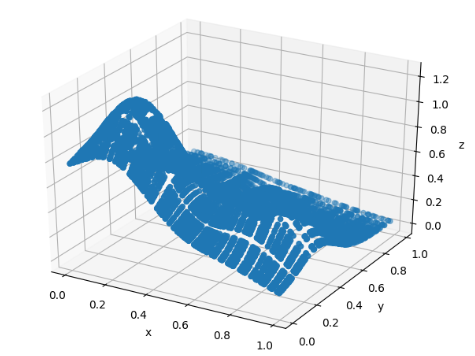
\includegraphics[width=7cm]{surface1}
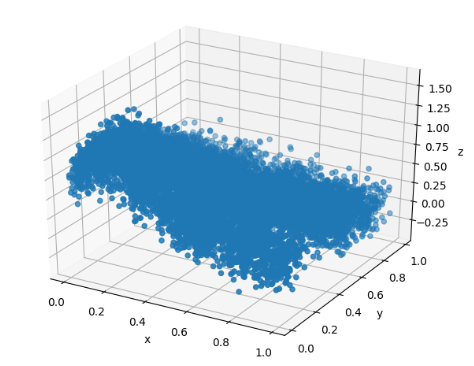
\includegraphics[width=7cm]{surfaceplusnoise}
\caption{Surfaces generated from sets x and y of 100 random numbers in the interval 0, 1, and set z from FrankeFunction [\ref{frankefunction}]}
\end{figure}

\subsubsection{Fitting the OLS model and predicting the targets}
\label{chap:Fitting the OLS model and predicting the targets}

\quad \, From the theory consolidated in Linear Regression's theory [\ref{chap:Linear Regression Theory}] of this report and using the created and pre-processed data by splitting [\ref{chap:Splitting data-set}] and scaling [\ref{chap:Scaling data-set}], we now develop an ordinary least squares algorithm to predict our target z (response vector).\\

In the \href{https://github.com/fabiorodp/UiO-FYS-STK4155/tree/master/Project1/package}{package/} directory, a file called \href{https://github.com/fabiorodp/UiO-FYS-STK4155/tree/master/Project1/package/linear_models.py}{linear\_models.py} contains an OLS class that performs the fitting, predictions, and confidence interval calculations.\\

First, initialize and fit OLS with X and z generated and pre-processed by \href{https://github.com/fabiorodp/UiO-FYS-STK4155/blob/master/Project1/package/Create_data.py}{CreateData} class, \href{https://scikit-learn.org/stable/modules/generated/sklearn.model_selection.train_test_split.html}{train\_test\_split(X, z, test\_size=0.2, random\_state=10)} and \href{https://scikit-learn.org/stable/modules/generated/sklearn.preprocessing.StandardScaler.html}{StandardScaler}.\\

The theory, described in [\ref{chap:Ordinary least squares}], explains how to find the expected coefficient vector beta while fitting the model. For that, the numpy linear algebra package does the computation job, such that:\\

\begin{lstlisting}[language=Python]
                numpy.linalg.pinv(X.T @ X) @ X.T @ z
\end{lstlisting}\\

After fitting OLS, the methods predict(X\_train) and predict(X\_test) performs the prediction for the training and testing data, respectively. Again, numpy linear algebra:\\

\begin{lstlisting}[language=Python]
                        X @ self.coef_
\end{lstlisting}\\

where x is X\_train or X\_test, and coef\_ is the vector of expected betas.\\

The confidence interval for the vector beta is described by the theory in [\ref{chap:Confidence Interval of the coefficients beta}] and coded as an OLS class method called \href{https://github.com/fabiorodp/UiO-FYS-STK4155/blob/master/Project1/package/Create_data.py}{coef\_confidence\_interval}.\\

Finally, we can assess the accuracy measures after predictions.\\

\subsubsection{Part A - Outputs and conclusion}
\label{chap:Part A - Outputs and conclusion}

\quad \, In this 'Part A' of our study, we ran our code for different polynomial transformations of degrees 2, 3, 4, 5, and for nr\_samples=12, and got as results the outputs present in the appendix [\ref{chap:Output - Part A}]. Also, one can run the file \href{https://github.com/fabiorodp/UiO-FYS-STK4155/blob/master/Project1/partA.py}{partA.py} to replicate the results.\\

For the training predictions, the outputs show MSE scores between 0.027 and 0.019, and R2-scores between 65 and 75 percent.\\

For the testing predictions, the outputs show MSE scores between 0.069 and 0.035 and R2-score between 65 and 77 percent.\\

Thus, the z\_train and z\_test predictions are near the real values. Also, the factors in the design matrix explain the target ($z$) at a rate of approx. 65 to 77 percent. Notice that as the polynomials' complexity increases from 2 to 5 as the r2-score increases and the MSE score decreases, it suggests that we could increase the polynomial degrees to acquire better results.\\

\subsection{Part B of the study}
\label{chap:Part B of the study}

\quad \, From Part A, we learned:\\

\quad \, - how to create the design matrix X and target z;\\ 

\quad \, - splitting and scaling the train and test sets;\\

\quad \, - fitting the linear regression model;\\

\quad \, - predicting the z-train and z-test targets;\\

\quad \, - evaluating the accuracy metrics MSE and r2-score.\\

Now, we will cover more specifics topics related to bias-variance trade-off and re-sampling techniques.\\

\subsubsection{Finding a benchmark for our study}
\label{chap:Finding a benchmark for our study}

\quad \, Before continuing our research, let's analyze a little more the OLS model's accuracy and find a benchmark for our study. Later on, we will try to beat this benchmark score using other linear regressions or machine learning techniques.\\

First, the file \href{https://github.com/fabiorodp/UiO-FYS-STK4155/blob/master/Project1/package/studies.py}{studies.py} located at \href{https://github.com/fabiorodp/UiO-FYS-STK4155/tree/master/Project1/package}{package/} directory contains a class function called GridSearch, which takes a range of values for both nr\_samples, poly\_degrees, and returns vectors of MSE and R2-score from all possible combinations of these two first input parameters.\\

Bellow, there is a printed output of a GridSearch of nr\_samples between 10 and 45, and poly\_degrees between 2 and 9:\\

\begin{figure}[H]
\label{fig:outputB1}
\centering
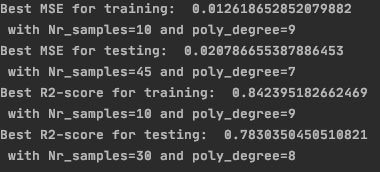
\includegraphics[width=8cm]{outputB1}
\caption{Output of the GridSearch for nr\_samples between 10 and 45, and poly\_degrees between 2 and 9.}
\end{figure}\\

One can see here that the best/minimal MSE obtained for training sets was approx. 0.012 for nr\_samples equals 10 and poly\_degree 9. On the other hand, for testing sets, the best/minimal MSE was 0.020 at nr\_samples 45 and poly\_degree 7.\\

In the same output, the best/maximal r2-score for training sets was approx. 0.84 at nr\_samples 10 and poly\_degree 9. For testing, it was 0.78 for nr\_samples 30 and poly\_degree 8.\\

These results show an accuracy improvement from the exercise partA [\ref{chap:Output - Part A}]. However, we need always to be cautious about under-fitting or over-fitting our model, as we can check more about it in the following heat-map plots:\\

\begin{figure}[H]
\label{fig:plotB1and2}
\centering
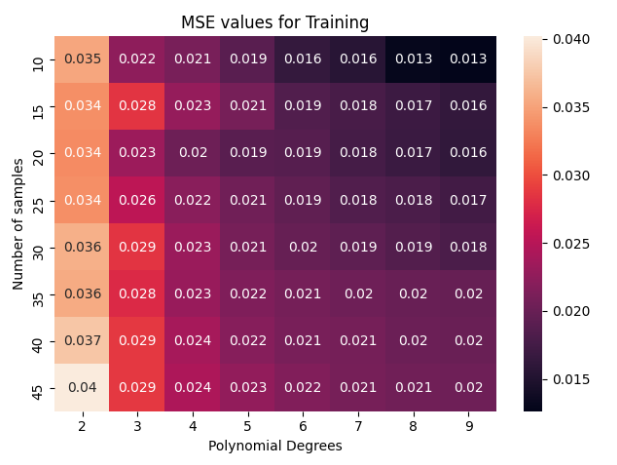
\includegraphics[width=7cm]{plotB1}
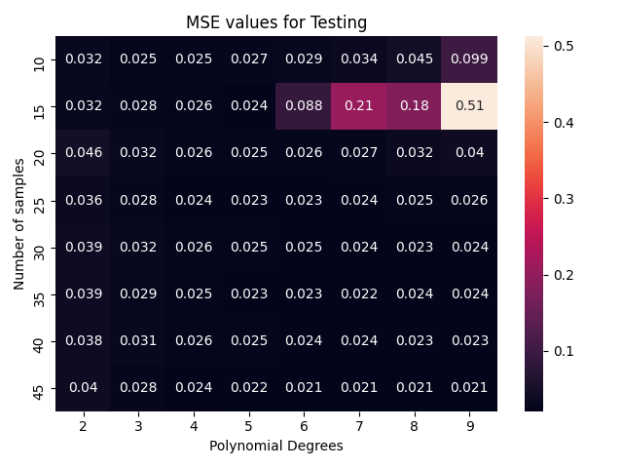
\includegraphics[width=7cm]{plotB2}
\caption{Heat-map containing the MSE train and test results of the GridSearch.}
\end{figure}\\

\begin{figure}[H]
\label{fig:plotB3and4}
\centering
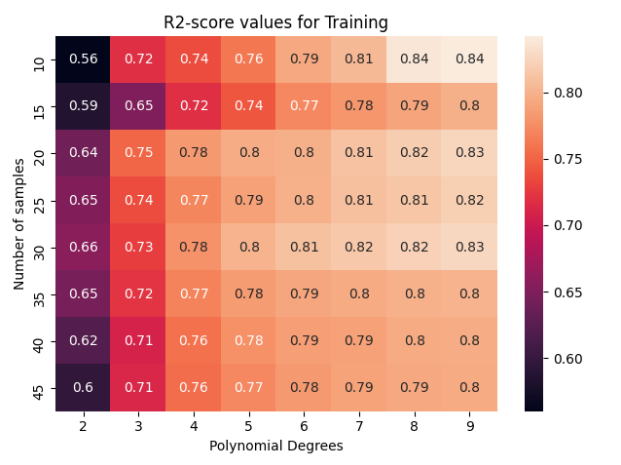
\includegraphics[width=7cm]{plotB3}
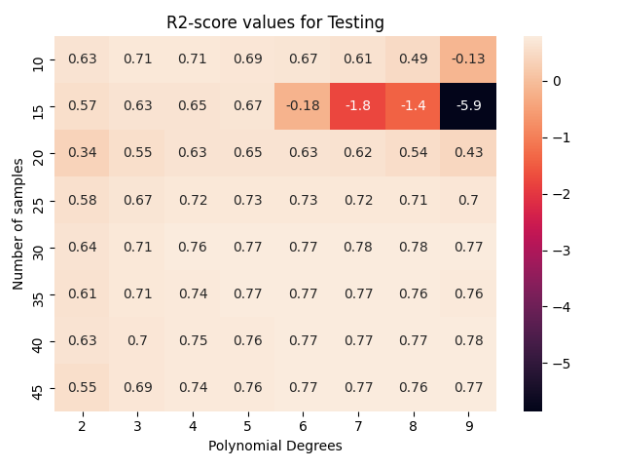
\includegraphics[width=7cm]{plotB4}
\caption{Heat-map containing the R2-score train and test results of the GridSearch.}
\end{figure}\\

From left to right, these heat-maps show that the accuracy of the predictions, for both metrics (MSE and R2-score), starts not desirable for a lower polynomial degree (under-fitting). As long as the polynomial degree increases, the metrics improve until a certain point and then worsen again (over-fitting).\\

The same happens when we take into consideration the top to the bottom of the heat-maps. The metrics start higher (under-fitting), and as long as the number of samples increases, the metrics improve until a certain point and then worsen again (over-fitting).\\

Let's analyze a similar plot as we can find in page 38 and 220 in \hyperref[Bib:TheElementsOfStatisticalLearningDataMining]{\textit{Hastie, Tibshirani, and Friedman}}, but with the data and parameters of our case:\\

\begin{figure}[H]
\label{fig:plotB5}
\centering
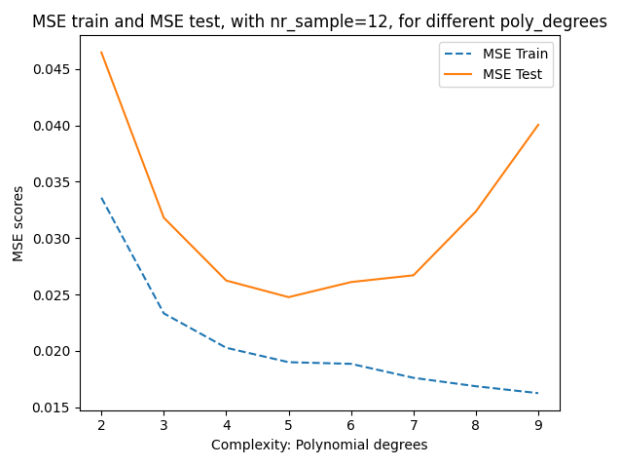
\includegraphics[width=8cm]{plotB5}
\caption{Line plots showing the MSE training and testing for parameters nr\_samples=20 and poly\_degrees from 2 to 9.}
\end{figure}\\

Notice that the plot's left side is a higher bias and lower variance region, the middle side is a lower bias and lower variance zone, and the right side is a higher bias and higher variance area. Hence, the sweet spot, for the complexity poly\_degree given nr\_sample=20, is around 4 or 5, where the testing MSE gets the best metric with low bias and variance plus closest to the training MSE.\\

As long as the complexity (poly\_degrees) increases, the scores get better values until a certain point, where after there is an expansion of the model's variance and the metrics worsen. This enlarged variance may indicate an over-fitting, which we will discuss in detail in the next subtopic.\\

For didactic purposes, we choose the number of samples equals 20 because there is an perfect behavior for visualizing the bias-variance trade-off decomposition.\\

Therefore, we choose our parameter nr\_sample equals 20 for our benchmark of this study.\\

\subsubsection{Bias-variance decomposition with bootstrapping technique} \\
\label{chap:Bias-variance decomposition with bootstrapping technique}

\quad \, Now, we can code an algorithm to illustrate the bias-variance trade-off decomposition as explained before in [\ref{chap:Bias-variance trade-off}] in more detail. For that, we use a re-sampling technique called bootstrapping. The file \href{https://github.com/fabiorodp/UiO-FYS-STK4155/blob/master/Project1/package/studies.py}{studies.py} in the \href{https://github.com/fabiorodp/UiO-FYS-STK4155/tree/master/Project1/package}{package/} directory has a class called BiasVarianceTradeOff that returns the decomposition and a plot. \\

The bootstrapping is a simple technique to re-sample the arguments X\_train and z\_train and predict each re-sampled response. \\

Let us analyze the plot for nr\_samples=20 and poly\_degrees between 2 and 8:

\begin{figure}[H]
\label{fig:plotB6}
\centering
\includegraphics[width=8cm]{plotb6}
\caption{Bias-variance decomposition for nr\_samples=20 and poly\_degrees between 2 and 8.}
\end{figure}\\

On the left side of the plot, there is a zone of high bias and low variance. As long the complexity polynomial degrees increases, the error and bias decrease until around poly\_degree=5. Then, the model's variance starts to increase, showing possible over-fitting, making the error metric sky rocket. Therefore, on the right side of the plot, there is a region of higher variance. \\

The sweet spot here, again, is when the polynomial degree is equal to 5. On this point, it is where the variance starts to increase significantly, and the error reaches the smallest score. \\

Thus, the poly\_degree=5 will be our benchmark in the next sections. \\

\subsubsection{Part B - Outputs and conclusion}
\label{chap:Part B - Outputs and conclusion}

\quad \, In this part, we studied the bias-variance trade-offs and its decomposition [\ref{chap:Bias-variance trade-off} and \ref{chap:Bias-variance decomposition with bootstrapping technique}]. Also, there was an implementation of a bootstrapping re-sampling model in file \href{https://github.com/fabiorodp/UiO-FYS-STK4155/blob/master/Project1/package/studies.py}{studies.py}. The output [\ref{chap:Output - Part B}] is in the appendix section of this report, and one can reproduce the code using the file \href{https://github.com/fabiorodp/UiO-FYS-STK4155/blob/master/Project1/partB.py}{partB.py}.\\

The  comparison  between  GridSearch  (partA)  and  bias-variance  trade-off with bootstrapping (partB) is below: \\

\begin{figure}[H]
\label{fig:compareB1}
\centering
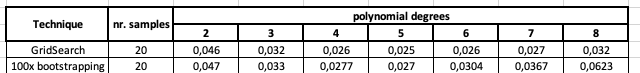
\includegraphics[width=15cm]{compareB1}
\caption{Comparison for testing MSE scores between techniques.}
\end{figure}\\

We see that the bootstrapping technique has not increased the precision of the MSE scores. This unimprovement might have occurred because the model already has enough data for training, then it is not necessary to re-sampling more data. Moreover, this bootstrapping increased the model's variance for higher polynomial degrees, which might infer that this re-sampling technique increased and accelerated our model's over-fitting. \\

\subsection{Part C of the study}
\label{chap:Part C of the study}

\quad \, This section will continue with Franke Function and Linear Regression study, but now applying a type of model selection called k-folds cross-validation. \\

\subsubsection{K-folds cross-validation to assess model performance}
\label{chap:K-folds cross-validation to assess model performance}

\quad \, To evaluate an acceptable bias-variance trade-off, we must carefully feed our model with specific training data to obtain reliable estimates on unseen samples. K-fold cross-validation is one of the well-known techniques that are widely implemented for this proposes. It splits the training data into k number of folds without replacement. One fold evaluates the predictions, and the others fit and train the machine learning model. This system is repeated k times so that we achieve k different models and estimate's scores. Then, these k scores return an estimated average performance of the model. \\

Typically, hyper-parameter tuning uses k-fold to assess generalization performances. The aim here is to provide more different pieces of training samples for the learning algorithm to obtain better-fitted models and more precise predictions. Also, it is an ideal method to tackle an insufficient number of samples in a data-set. \\

An excellent drawing, that summarizes the k-folds systems, is present on page 299 of the book \hyperref[Bib:PythonMachineLearning]{\textit{Python Machine Learning}} \hyperref[Bib:PythonMachineLearning]{[S. Raschka, V. Mirjalili]}, which is replicated here: \\

\begin{figure}[H]
\label{fig:figC1}
\centering
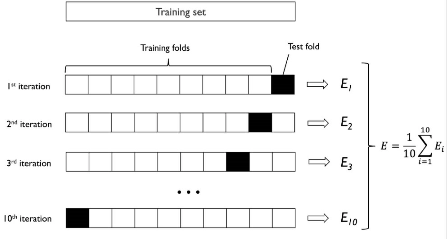
\includegraphics[width=8cm]{figC1}
\caption{K-fold cross-validation system.}
\end{figure}\\

The file \href{https://github.com/fabiorodp/UiO-FYS-STK4155/blob/master/Project1/package/studies.py}{studies.py} in the \href{https://github.com/fabiorodp/UiO-FYS-STK4155/tree/master/Project1/package}{package/} directory has a class called CrossValidationKFolds that performs this system explained above. \\

Then, let's implement this technique for 5-10 folds with 20 samples and polynomial degrees 2-8: \\

\begin{figure}[H]
\label{fig:plotC1-2}
\centering
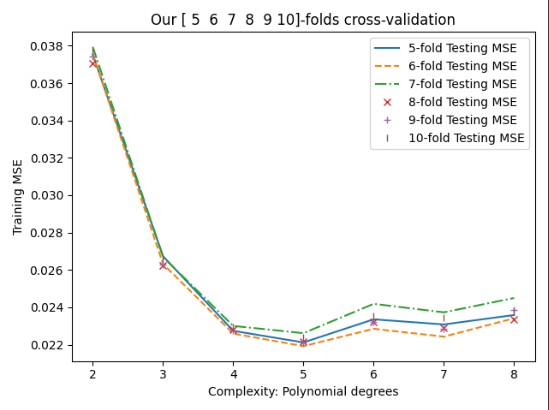
\includegraphics[width=7cm]{plotC1}
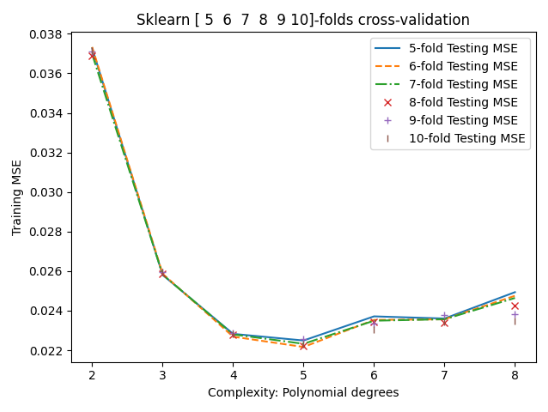
\includegraphics[width=7cm]{plotC2}
\caption{The left side plot is our algorithm for k-folds where k=[5, 6, 7, 8, 9, 10], nr\_samples=20 and poly\_degrees=[2, 3, 4, 5, 6, 7, 8]. The right side plot is a Scikit-Learn k-fold algorithm with the same parameters, but using the Linear Regression model from Sci-kit.}
\end{figure}\\

Notice that our algorithms and Sci-kit's algorithms have quite the same outputs. \\

The k-folds brought an attenuation in the testing MSE indications. This mitigation might have occurred because of the reduction of the model's variance. Besides, the sample space of the training data is smaller as the number of folds is higher, then it could have decreased the complexity of the model and, therefore, the variance. \\

\subsubsection{Part C - Outputs and conclusion}
\label{chap:Part C - Outputs and conclusion}

\quad \, In this part, we studied the k-folds Cross-Validation technique. Also, there was our implementation of k-folds cross-validation in file \href{https://github.com/fabiorodp/UiO-FYS-STK4155/blob/master/Project1/package/studies.py}{studies.py}. The outputs are in this report's appendix section [\ref{chap:Output - Part C}]. Also, the experiment can be reproduced by the file \href{https://github.com/fabiorodp/UiO-FYS-STK4155/blob/master/Project1/partC.py}{partC.py} in our GitHub repository.\\

The comparison among GridSearch (partA), bias-variance trade-off with bootstrapping (partB) and k-folds cross-validation (partC) is below: \\

\begin{figure}[H]
\label{fig:compareC1}
\centering
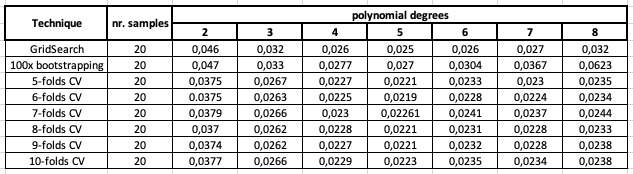
\includegraphics[width=15cm]{compareC1}
\caption{Comparison for testing MSE scores between techniques.}
\end{figure}\\

We see that the k-folds cross-validation technique has improved the testing MSE scores. This improvement might have occurred because of the sample space of the training data, which is smaller as the number of folds is higher, then it might have decreased the complexity of the model and, therefore, the variance.\\

\subsection{Part D of the study}
\label{chap:Part D of the study}

\quad \, This section will continue with Franke's function [\ref{frankefunction}], but now applying a different linear regression model called Ridge Regression [\ref{chap:Ridge Regression}]. We will also optimize the Ridge's hyper-parameter lambda, performing bootstrapping and k-folds cross-validation. In the end, it will be checked if there is any improvement in the testing MSE scores while using its shrinkage regularization.\\

\subsubsection{Ridge's hyper-parameter lambda - Regularization}
\label{chap:Ridge's hyper-parameter lambda - Regularization}

\quad \, As studied in the section about linear regression theory [\ref{chap:Ridge Regression}], Ridge Regression aims to attenuate the OLS model's variance by introducing a regularization technique. This new parameter, $\lambda >= 0$, is added at the end of the OLS's cost function, enabling tuning the optimum betas and variance. \\

The heat-map below illustrates the higher lambda, the lower coefficients of the linear regression (betas) are: \\

\begin{figure}[H]
\label{fig:heatmapD1}
\centering
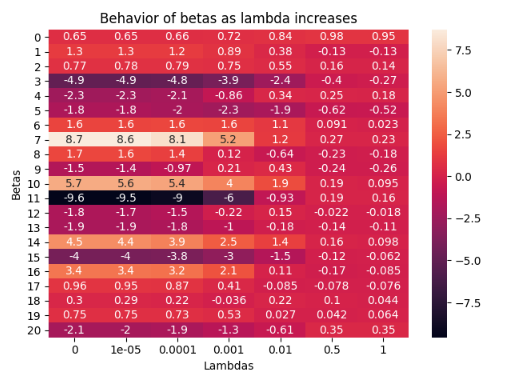
\includegraphics[width=8cm]{heatmapD1}
\caption{Heat-map showing the behavior of betas as lambda increases for nr\_samples=20 and poly\_degree=5.}
\end{figure} \\

As said before, this reduction of the betas attenuates the variance by diminishing the over-fitting. On the other hand, we have to be careful when using the lambda because very high lambda under-fits the model. This under-fit occurs because of reducing the betas, which might bring lower complexity for the model.\\

\subsubsection{GridSearch for finding the best Ridge's lambda} \\
\label{chap:GridSearch for finding the best Ridge's lambda}

\quad \, Now, it is time to find the best lambda value for our data-sets with sample space of 20 (nr\_samples parameter). For that, a GridSearch is run:\\

\begin{figure}[H]
\label{fig:heatmapD2andD3}
\centering
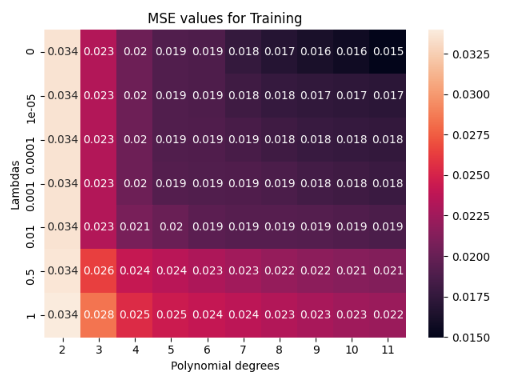
\includegraphics[width=7cm]{heatmapD2}
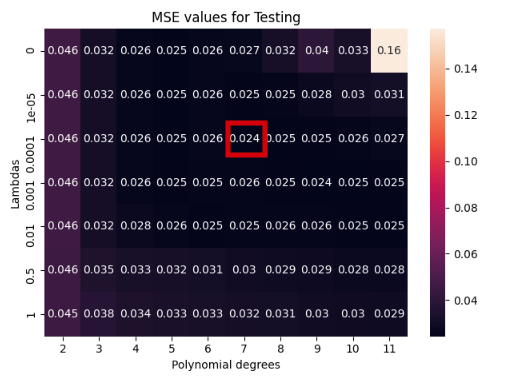
\includegraphics[width=7cm]{heatmapD3}
\caption{Heat-maps showing the behavior of training (left) and testing (right) MSE scores as lambda and polynomial degrees increase.}
\end{figure}\\

\begin{figure}[H]
\label{fig:heatmapD4andD5}
\centering
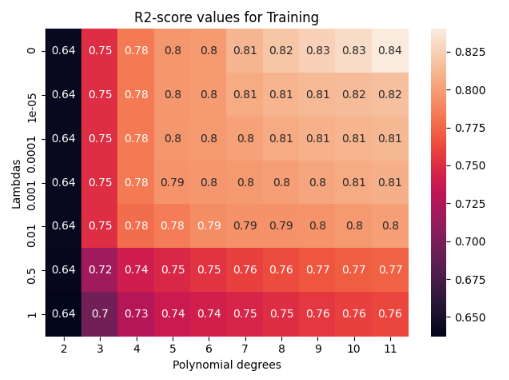
\includegraphics[width=7cm]{heatmapD4}
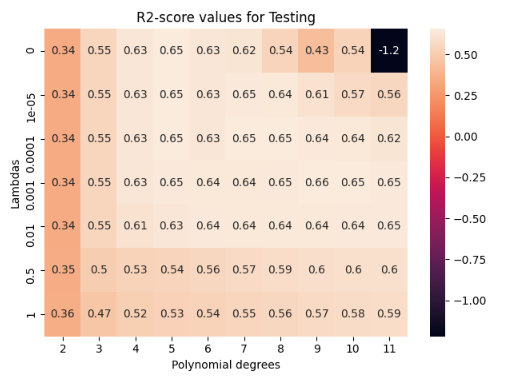
\includegraphics[width=7cm]{heatmapD5}
\caption{Heat-maps showing the behavior of training (left) and testing (right) R2-scores as lambdas and polynomial degrees increase.}
\end{figure}\\

Here, we are interested in finding the best MSE testing score for as lower complexity as possible, where it is seen at lambda equals 0,0001, and polynomial degree equals 7.\\

Notice, also, that where $\lambda=0$ means that the Ridge model is equal to the OLS model. Thus, as expected, as long as the lambda increases, the variance for higher polynomial degrees decreases compared to the OSL model. \\

Therefore, lambda equals to 0,0001 is chosen for studying the training and testing MSE plot below: \\

\begin{figure}[H]
\label{fig:MSEplotD1}
\centering
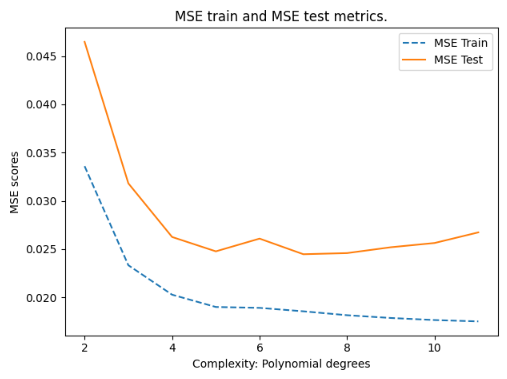
\includegraphics[width=8cm]{MSEplotD1}
\caption{Line plot showing the behavior of training and testing MSE-scores for lambda=0.0001, number of samples equals 20 and polynomial degrees between 2, 12.}
\end{figure}\\

As expected,  there is a lower variance for a higher polynomial degree than the OLS's plot [\ref{fig:plotB5}], with the same parameters. \\

\subsubsection{Ridge's Bias-variance trade-off with bootstrapping}
\label{chap:Ridge's Bias-variance trade-off with bootstrapping}

\quad \, Here, it was performed a 100x bootstrapping for studying the bias-variance trade-off. For that, we set lambda=0.0001, nr\_samples=20, and poly\_degrees from 2 to 12: \\

\begin{figure}[H]
\label{fig:BiasplotD2}
\centering
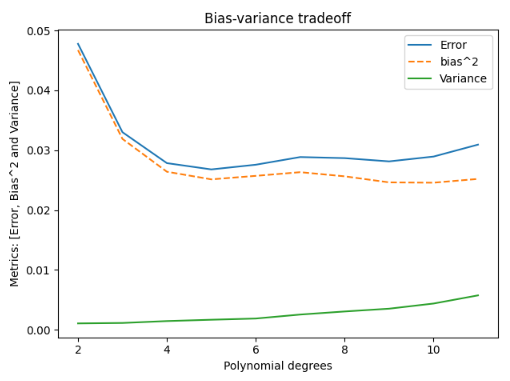
\includegraphics[width=8cm]{plotD2}
\caption{Line plot showing the bias-variance trade-off.}
\end{figure}\\

As expected again, there is a lower variance for a higher polynomial degree than the OLS's plot [\ref{fig:plotB6}], with the same parameters.\\

\subsubsection{Ridge's k-folds cross-validation}
\label{chap:Ridge's k-folds cross-validation}

\quad \, We continue with 20 for the number of samples and 0,0001 for lambda and, finally, run the k-folds cross-validation for polynomial degrees between 2 to 12:\\

\begin{figure}[H]
\label{fig:plotD3andh6}
\centering
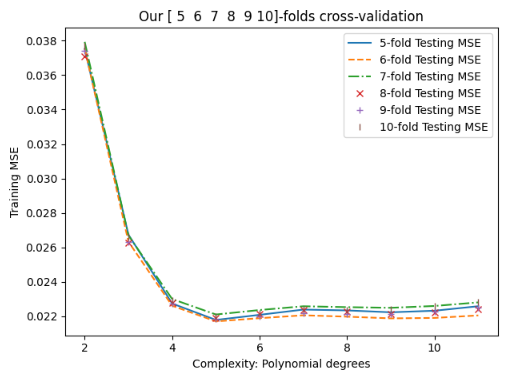
\includegraphics[width=7cm]{plotD3}
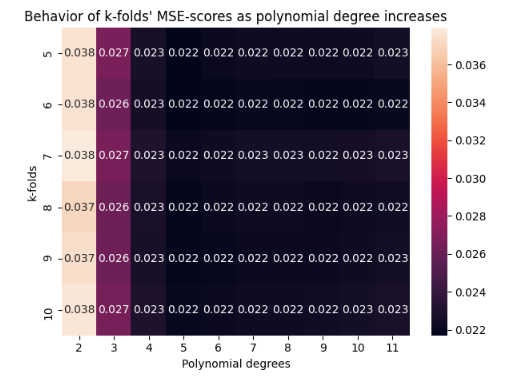
\includegraphics[width=7cm]{heatmapD6}
\caption{Left side containing line plots for different k-folds. Right side containing heat-map with the k-folds' MSE results.}
\end{figure}\\

Again, one can observe that the model's variance takes longer to appear, and the plots have more stable lines. \\

\subsubsection{Part D - Outputs and conclusions}
\label{chap:Part D - Outputs and conclusions}

\quad \, In this part, we studied the GridSearch, bias-variance trade-offs, and k-folds cross-validation techniques for Ridge regression. The outputs are in this report's appendix section [\ref{chap:Output - Part D}]. The experiment can be reproduced by using the file \href{https://github.com/fabiorodp/UiO-FYS-STK4155/blob/master/Project1/partD.py}{partD.py} in our GitHub repository.\\

The comparison among GridSearch (partA), bias-variance trade-off with bootstrapping (partB) and k-folds cross-validation (partC) is below:\\

\begin{figure}[H]
\label{fig:comparisonD}
\centering
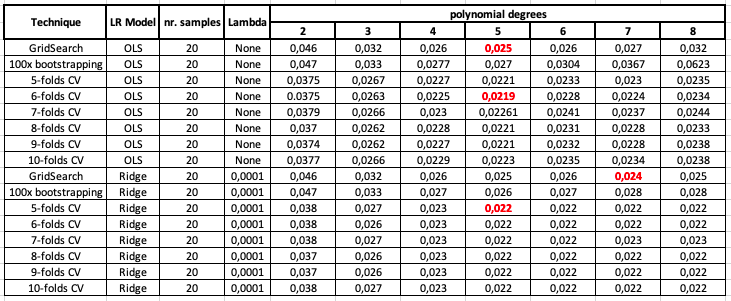
\includegraphics[width=15cm]{comparisonD}
\caption{Comparison for testing MSE scores between techniques.}
\end{figure}\\

The best testing MSE achieved with Ridge was 0,022 for 5-folds cross-validation. On the other hand, the best score for testing MSE with the OLS model was 0,0219 for 6-folds cross-validations.\\

Even though the Ridge regression reduced the predictions' variance, it did not reach a better score than the OLS model for polynomial degrees between 2-8.\\

Ridge regression makes it possible to increase the polynomial degrees (complexity of the model) with lower variance than OLS; then, it might be beneficial and might get better scores if a higher degree is applied.\\

\subsection{Part E of the study}
\label{chap:Part E of the study}

\quad \, This section will apply a new linear regression model called Lasso. We will also optimize the Lasso's hyper-parameter lambda, performing bootstrapping and k-folds cross-validation. In the end, it will be checked if there is any improvement in the testing MSE scores while using its regularization. \\

\subsubsection{Lasso's hyper-parameter lambda - Regularization}
\label{chap:Lasso's hyper-parameter lambda - Regularization}

\quad \, As studied in the section about Lasso's theory [\ref{chap:Lasso Regression}], the aim here is to attenuate the OLS model's variance by introducing a regularization technique. This regularization penalizes the regression's betas, the ones with less relevance for the predictions, forcing them to converge to its minimum.\\

As we did for Ridge's model, but now for Lasso's, the heat-map below illustrates the higher lambda, the lower coefficients of the linear regression (betas) are: \\

\begin{figure}[h]
\label{fig:heatmapE1}
\centering
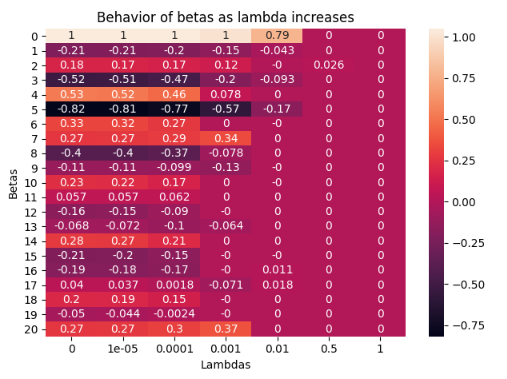
\includegraphics[width=8cm]{heatmapE1}
\caption{Heat-map showing the behavior of betas as lambda increases for nr\_samples=20 and poly\_degree=5}
\end{figure}\\

Notice that when lambda is 0, the Lasso model has the same coefficients as the OLS's model. Also, we have to be careful when using the lambda because very high lambda under-fits the model. From the heat-map, lambda equals one results in all coefficients 0, which ends up in an under-fitted model with very low complexity.\\

\subsubsection{Finding the best lambda with GridSearch}
\label{chap:Finding the best lambda with GridSearch}

\quad \, A GridSearch finds the best lambda's value for our data-sets: \\

\begin{figure}[H]
\label{fig:heatmapE2andE3}
\centering
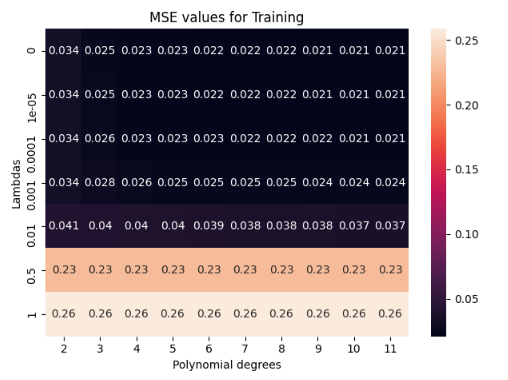
\includegraphics[width=7cm]{heatmapE2}
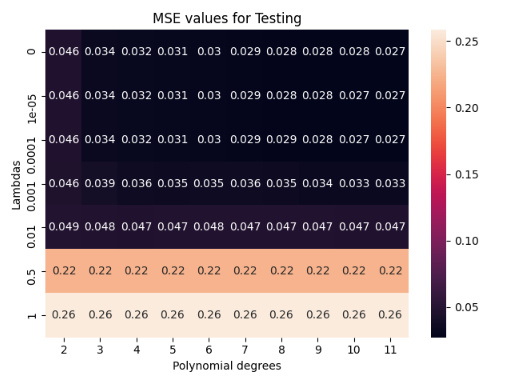
\includegraphics[width=7cm]{heatmapE3}
\caption{Heat-maps showing the behavior of training (left) and testing (right) MSE scores as lambda and polynomial degrees increase.}
\end{figure}\\

\begin{figure}[H]
\label{fig:heatmapE4andE5}
\centering
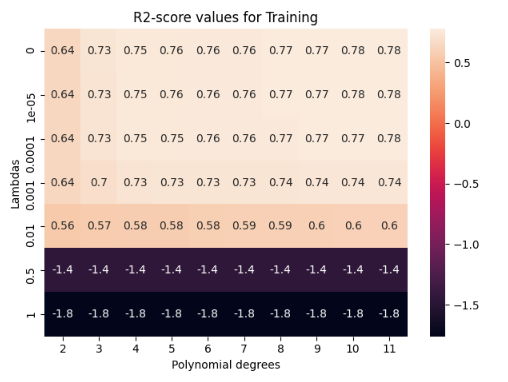
\includegraphics[width=7cm]{heatmapE4}
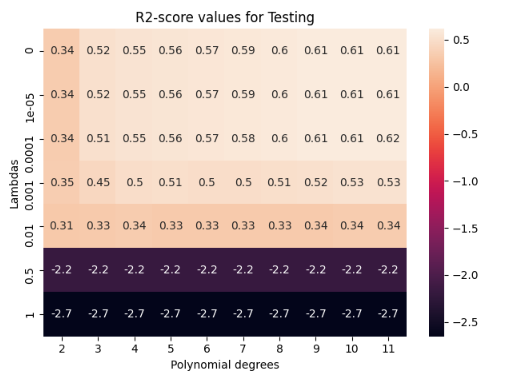
\includegraphics[width=7cm]{heatmapE5}
\caption{Heat-maps showing the behavior of training (left) and testing (right) R2-scores as lambdas and polynomial degrees increase.}
\end{figure}\\

Hence, as expected and similar to Ridge's model, as long as the lambda increases, the variance for higher polynomial degrees decreases compared to the OSL's model. \\

Lambda equals to 0,0001 is chosen for studying the training and testing MSE plot below: \\

\begin{figure}[H]
\label{fig:plotE1}
\centering
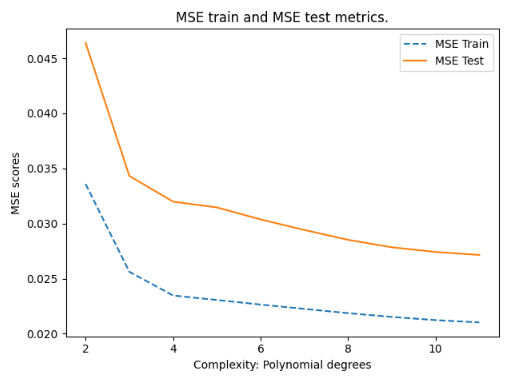
\includegraphics[width=8cm]{plotE1}
\caption{Line plot showing the behavior of training and testing MSE-scores for lambda=0.0001, number of samples equals 20 and polynomial degrees between 2, 12.}
\end{figure}\\

There is still a lower variance for a higher polynomial degree than the OLS's plot [\ref{fig:plotB5}] and quite the same as Ridge's [\ref{fig:MSEplotD1}].\\

\subsubsection{Lasso's Bias-variance trade-off with bootstrapping}
\label{chap:Lasso's Bias-variance trade-off with bootstrapping}

\quad \, It was performed a 100x bootstrapping for studying the bias-variance trade-off. For that, we set lambda=0.0001, nr\_samples=20, and poly\_degrees from 2 to 12:\\

\begin{figure}[H]
\label{fig:BiasplotE2}
\centering
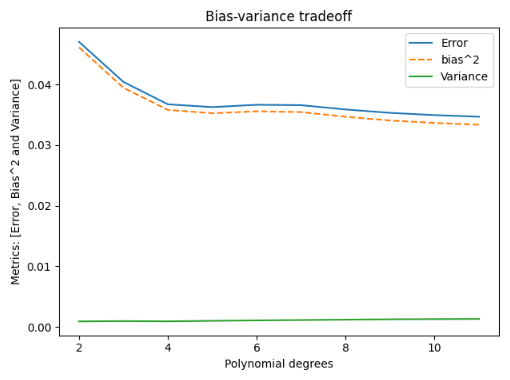
\includegraphics[width=8cm]{plotE2}
\caption{Line plot showing the bias-variance trade-off.}
\end{figure}\\

The decomposition of the bias-variance trade-off shows a lower variance for a higher polynomial degree than the OLS's [\ref{fig:plotB6}] and Ridge's plot [\ref{fig:BiasplotD2}], with the same parameters.\\

\subsubsection{Lasso's k-folds cross-validation}
\label{chap:Lasso's k-folds cross-validation}

\quad \, For nr\_samples=20 and lambda=0,0001, we run the k-folds cross-validation for polynomial degrees between 2 to 12:

\begin{figure}[H]
\label{fig:plotE3andh6}
\centering
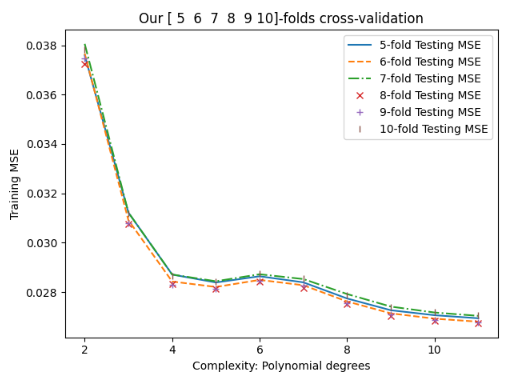
\includegraphics[width=7cm]{plotE3}
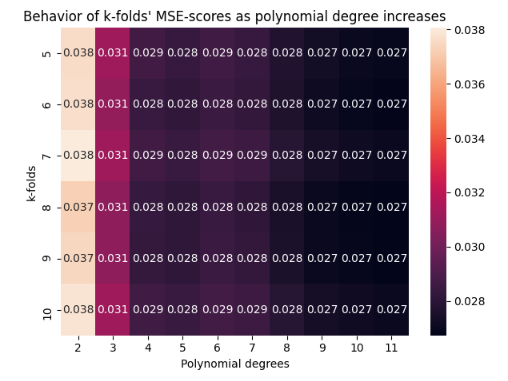
\includegraphics[width=7cm]{heatmapE6}
\caption{Left side containing line plots for different k-folds. Right side containing heat-map with the k-folds' MSE results.}
\end{figure}\\

Notice that the MSE values converge to its minimum for all k-folds numbers.\\

\subsubsection{Part E - Outputs and conclusions}
\label{chap:Part E - Outputs and conclusions}

\quad \, In this part, we studied Lasso's regression model by introducing GridSearch, bias-variance trade-offs with bootstrapping, and k-folds cross-validation. The outputs are in this report's appendix section [\ref{chap:Output - Part E}]. The experiment can be reproduced by using the file \href{https://github.com/fabiorodp/UiO-FYS-STK4155/blob/master/Project1/partE.py}{partE.py} in our GitHub repository.\\ 

The comparison among GridSearch (partA), bias-variance trade-off with bootstrapping (partB) and k-folds cross-validation (partC) is below:\\

\begin{figure}[H]
\label{fig:comparisonE}
\centering
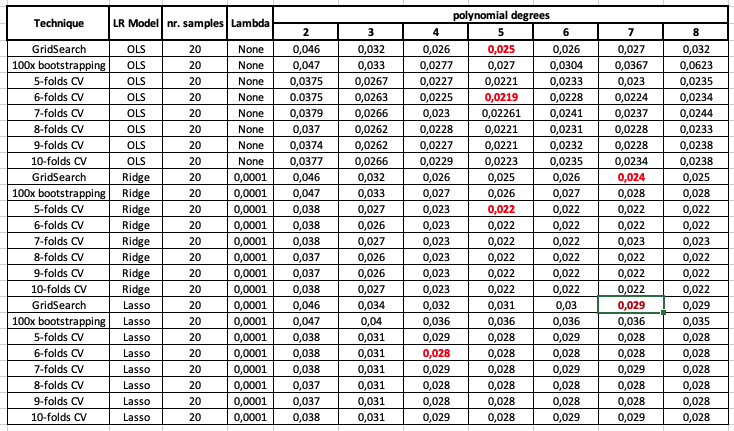
\includegraphics[width=15cm]{comparisonE}
\caption{Comparison for testing MSE scores between techniques.}
\end{figure}\\

The best testing MSE achieved with Lasso was 0,028 for 6-folds cross-validation, which is worse than OLS's and Ridge's performances.\\

Lasso regression makes it possible to increase the polynomial degrees (complexity of the model) with lower variance than OLS; then, it might be beneficial and might get better scores if we increase the model's complexity.\\

\subsection{Part F and G of the study}
\label{chap:Part F and G of the study}

\quad \, This section will apply all the subjects studied before on real terrain heights. For that, we downloaded a GeoTIF file from \href{https://earthexplorer.usgs.gov/}{https://earthexplorer.usgs.gov/}, containing specific altitudes of a region near Stavanger in Norway, and stored it in the directory \href{https://github.com/fabiorodp/UiO-FYS-STK4155/tree/master/Project1/data}{data/}. The visualization of this region is plotted below: \\

\begin{figure}[H]
\label{fig:imageF}
\centering
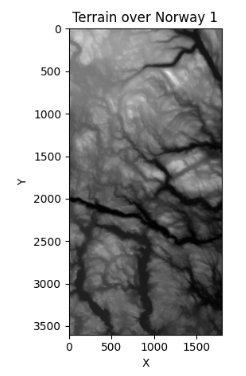
\includegraphics[width=4cm]{imageF}
\caption{Terrain heights plot from a GeoTIF file.}
\end{figure}\\

\subsubsection{OLS model on terrain data}
\label{chap:OLS model on terrain data}

\quad \, We utilize the same polynomial transformation method used in the previous exercises to generate our explanatory variables x and y. The response variable z will be the heights extracted from the GeoTIF file downloaded. We also slice the original image to a smaller fraction to avoid expensive computational calculations and run a GridSearch to analyze the behavior of the MSE score and R2-score under the OLS model:\\

\begin{figure}[H]
\label{fig:heatmapF1and2}
\centering
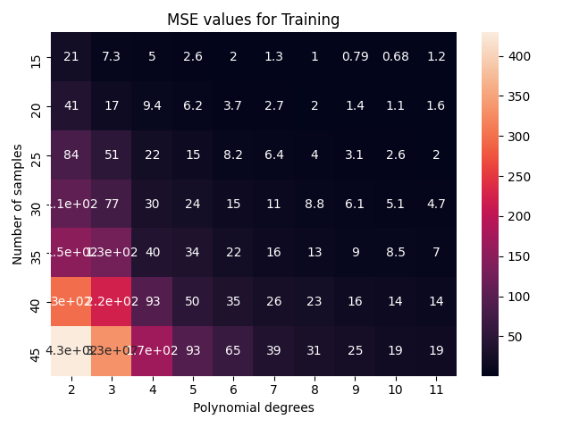
\includegraphics[width=7cm]{heatmapF1}
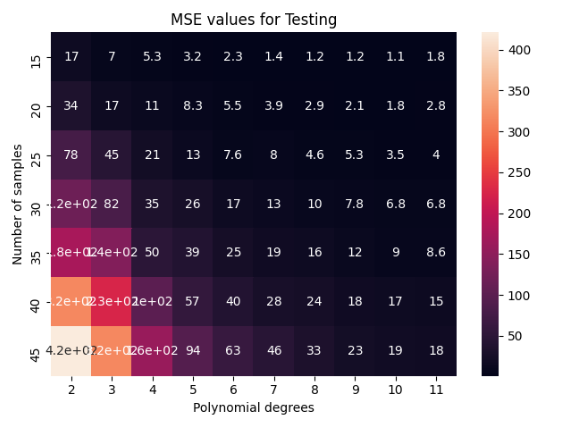
\includegraphics[width=7cm]{heatmapF2}
\caption{Heat-map with the training (left) and testing (right) MSE scores for the terrain's heights using OLS model.}
\end{figure}\\

\begin{figure}[H]
\label{fig:heatmapF3and4}
\centering
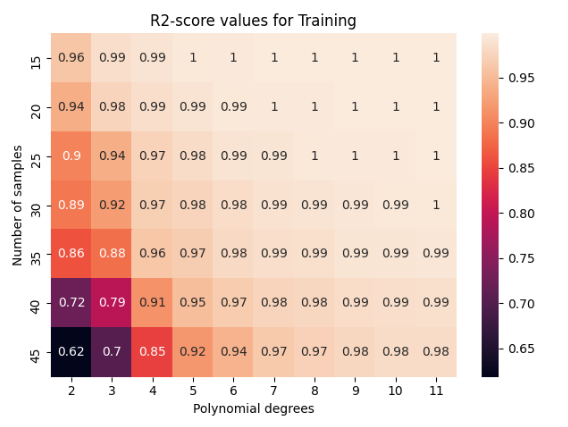
\includegraphics[width=7cm]{heatmapF3}
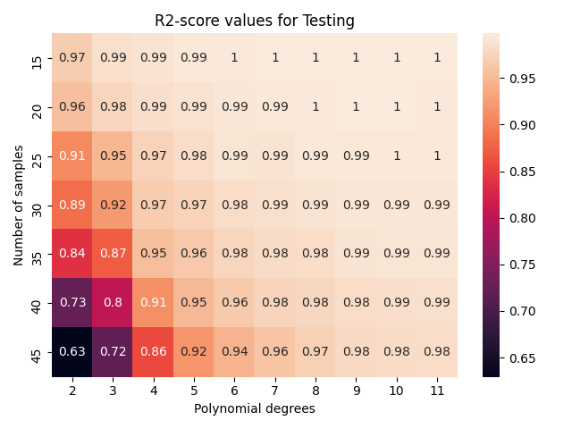
\includegraphics[width=7cm]{heatmapF4}
\caption{Heat-map with the training (left) and testing (right) R2-score for the terrain's heights using OLS model.}
\end{figure}\\

One can see that the predictions are more accurate when the image/region is smaller. As long the picture gets larger, the precision decreases, but with still a very high R2-score. This behavior means that our regression model does a better job predicting smaller regions than bigger ones with higher complexities. Besides, high R2-scores means that the explanatory variables do a very good job explaining the response variable, in a rate of approximately 60-90 percent in these heat-map cases.\\

Notice, we can also improve MSE performance for larger pictures by increasing the polynomial degree. However, it will become significantly computational expensive. Thus, for didactic propose, the size of the image is chosen at 15 nr\_samples.\\

Following are the results for the training and testing MSE scores, the decomposition of the bias-variance trade-offs with bootstrapping and k-folds cross-validation:\\

\begin{figure}[H]
\label{fig:plotF1andF2}
\centering
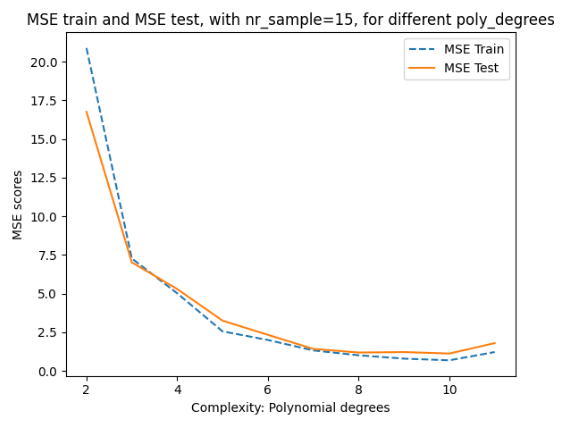
\includegraphics[width=7cm]{plotF1}
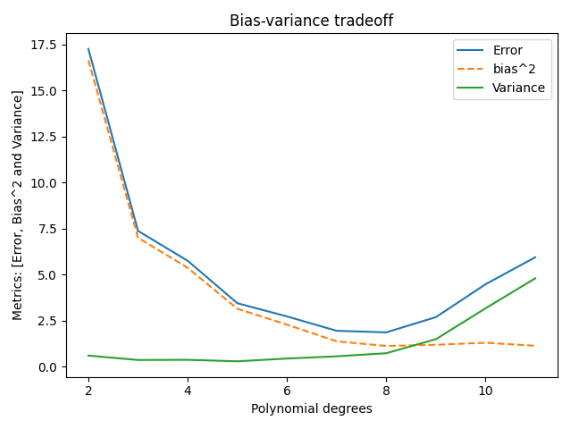
\includegraphics[width=7cm]{plotF2}
\caption{Left-side containing a line-plot for training and testing MSE. Right-side with the bias-variance decomposition with 100x bootstrapping.}
\end{figure}\\

\begin{figure}[H]
\label{fig:plotF3andH5}
\centering
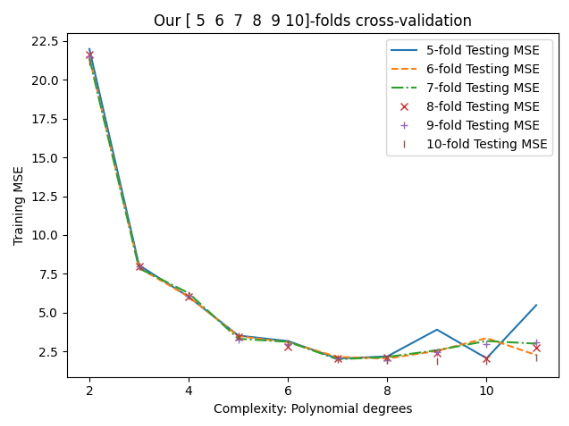
\includegraphics[width=7cm]{plotF3}
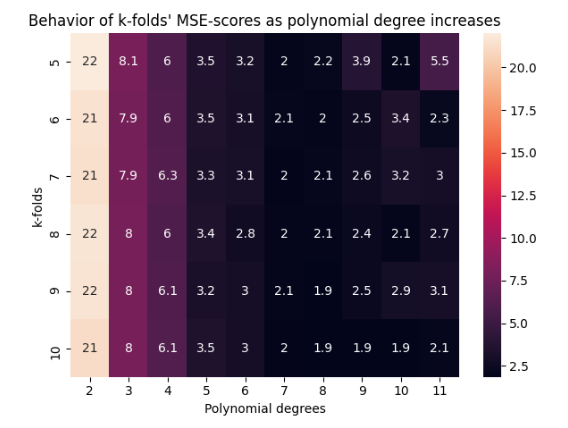
\includegraphics[width=7cm]{heatmapF5}
\caption{Left-side with k-folds' cross-validation line plots. Right-side containing k-folds' cross-validation results.}
\end{figure}\\

From the left-side of figure 29, the best testing MSE is 1.1 for a polynomial degree 10. However, from the right side of figure 29, this 1.1 result might be over-estimated because the bias-variance trade-off shows a significant increase in the variance of the model at polynomial degree 7. This supposed over-estimation is also confirmed by the k-folds cross-validation line-plot and heat-map, in figure 30, where the best testing MSE was obtained with a lower polynomial degree around 7 or 8. \\

A break-down of the study-results can be checked below: \\

\begin{figure}[H]
\label{fig:comparisonF1}
\centering
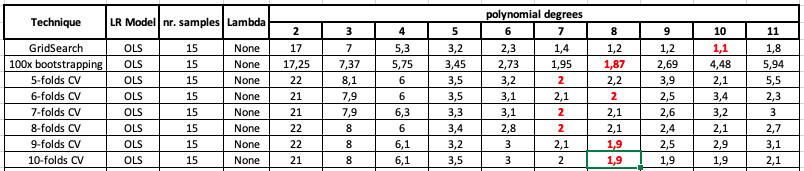
\includegraphics[width=15cm]{comparisonF1}
\caption{Break-down of the results among studies.}
\end{figure}\\

The conclusion one can obtain from these results is that, for a small picture/region sliced with only 15 samples, we obtain the sweet-spot of the predictions around polynomial of 7 or 8 degrees. Over that, the model starts to over-fits with a significant increase in the variance. Under that, the models under-fits because of the lack of information.\\

\subsubsection{Ridge model on terrain data}
\label{chap:Ridge model on terrain data}

\quad \, This experiment utilizes the same polynomial transformation used before to generate the design matrix X. Also, the targets z are the heights from the GeoTIF picture. However, this research focuses on the Ridge regression, especially finding the best regularization or the optimum parameter lambda's best value.\\

For that, the algorithm named \href{https://github.com/fabiorodp/UiO-FYS-STK4155/blob/master/Project1/partFandG.py}{partFandG.py} in our Github repository directory \href{https://github.com/fabiorodp/UiO-FYS-STK4155/blob/master/Project1/}{Project1/} does the calculations job for us, such that:\\

\begin{figure}[H]
\label{fig:heatmapFR1and2}
\centering
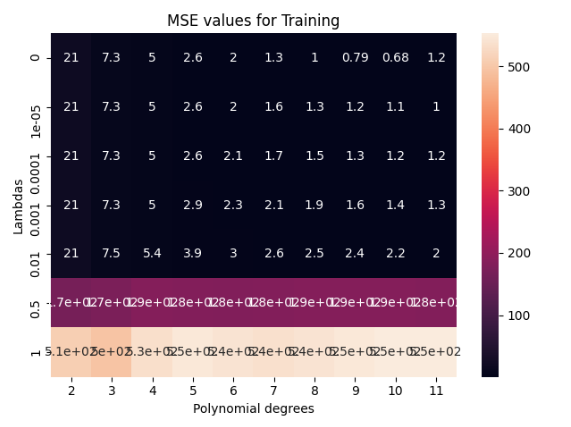
\includegraphics[width=7cm]{heatmapFR1}
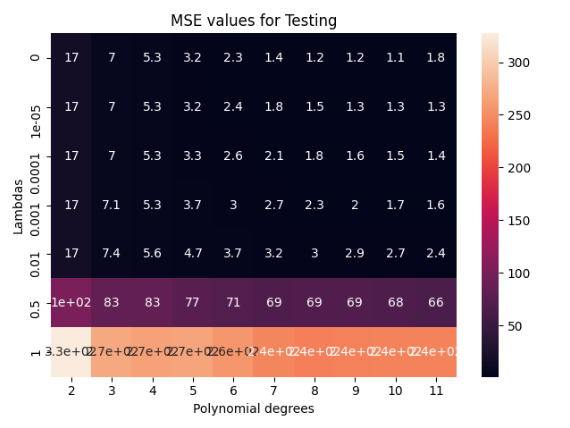
\includegraphics[width=7cm]{heatmapFR2}
\caption{Left-side containing a heat-map with training MSE scores for different polynomial degrees and lambdas. Right-side containing a heat-map with testing MSE scores for different polynomial degrees and lambdas.}
\end{figure}\\

\begin{figure}[H]
\label{fig:heatmapFR3and4}
\centering
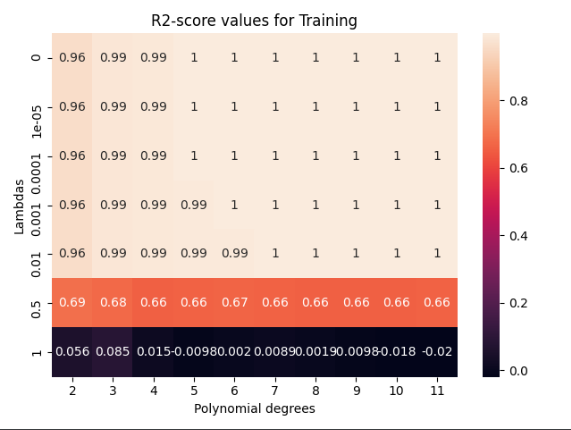
\includegraphics[width=7cm]{heatmapFR3}
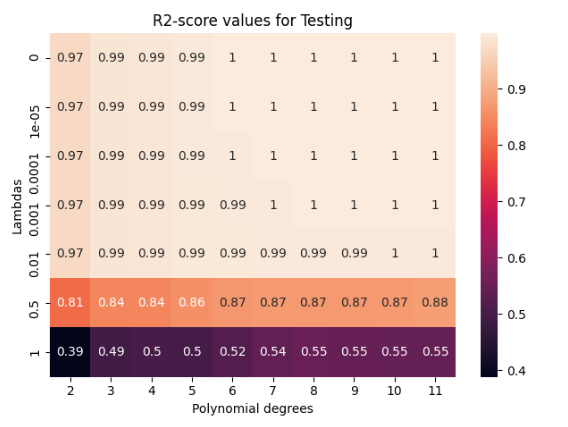
\includegraphics[width=7cm]{heatmapFR4}
\caption{Left-side containing a heat-map with training R2 scores for different polynomial degrees and lambdas. Right-side containing a heat-map with testing R2 scores for different polynomial degrees and lambdas.}
\end{figure}\\

The significant difference here from the heat-maps for the OLS model [\ref{fig:heatmapF1and2}] is that Ridge regression with regularization enables us to get a higher polynomial degree without over-estimate the predictions. For instance, the OSL model reaches its minimum testing scores at polynomial degrees around 8-10 for lambda 0.0001; on the other hand, the Ridge's testing score, with the same parameters, is still decreasing, showing that the variance has not increased yet. \\

Let us see the bias-variance decomposition for 100x bootstrapping and k-folds cross-validation: \\

\begin{figure}[H]
\label{fig:plotFR1and2}
\centering
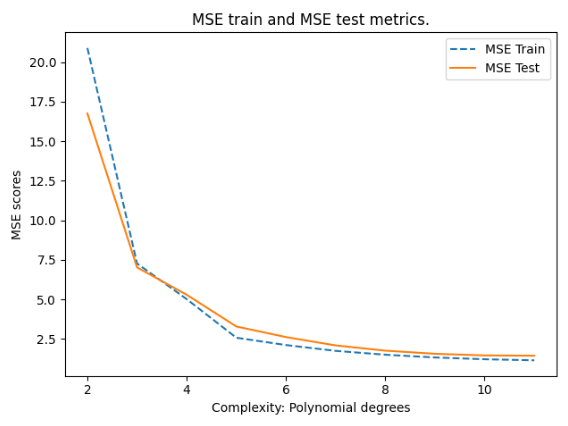
\includegraphics[width=7cm]{plotFR1}
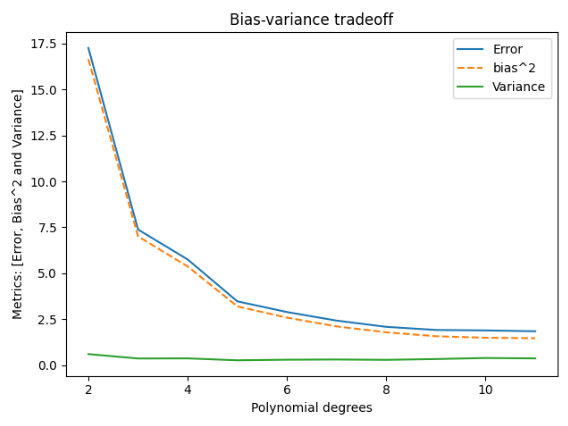
\includegraphics[width=7cm]{plotFR2}
\caption{Left-side containing a line-plot with training and testing MSE scores for different polynomial degrees, and lambda=0.0001. Right-side containing a line-plot with the decomposition of the bias-variance with 100x bootstrapping, for different polynomial degrees, and lambda=0.0001.}
\end{figure}\\

\begin{figure}[H]
\label{fig:plotFR3andH5}
\centering
\includegraphics[width=7cm]{plotFR3}
\includegraphics[width=7cm]{heatmapFR5}
\caption{Left-side containing a line-plot with testing MSE scores for different polynomial degrees and k-folds, and lambdas=0.0001. Right-side containing a heat-map with testing MSE scores for different polynomial degrees and k-folds, and lambda=0.0001.}
\end{figure}\\

From figure 34, the variance has slowly started to increase at polynomial's degree 10, but much less than in the same circumstance at the OLS's model [\ref{fig:plotF1andF2}]. Besides, the Ridge's testing MSE is still descending towards its minimum at polynomial 11, in contrast to the OLS's model [\ref{fig:plotF1andF2}], where its minimum had already occurred.\\

Figure 35 confirms what was said; the scores are still going towards its minimum at polynomial degree 10-11; however, they have better metrics than the bootstrapping technique because it slightly reduces the model's complexity when dividing the samples into groups of k-folds.\\

Therefore, for comparison propose, a table with scores between the OLS model and Ridge model is stated as follows: \\

\begin{figure}[H]
\label{fig:comparisonF2}
\centering
\includegraphics[width=15cm]{comparisonF2}
\caption{Break-down of the results among studies.}
\end{figure}\\

\subsubsection{Lasso model on terrain data}
\label{chap:Lasso model on terrain data}

\quad \, This last practice will utilize the Lasso linear regression model with the same parameters, design matrix, and targets used in the previous sections. \\

For that, the algorithm named \href{https://github.com/fabiorodp/UiO-FYS-STK4155/blob/master/Project1/partFandG.py}{partFandG.py} in our Github repository directory \href{https://github.com/fabiorodp/UiO-FYS-STK4155/blob/master/Project1/}{Project1/} does the calculations job for us, such that: \\

\begin{figure}[H]
\label{fig:heatmapFL1and2}
\centering
\includegraphics[width=7cm]{heatmapFL1}
\includegraphics[width=7cm]{heatmapFL2}
\caption{Left-side containing a heat-map with training MSE scores for different polynomial degrees and lambdas. Right-side containing a heat-map with testing MSE scores for different polynomial degrees and lambdas.}
\end{figure}\\

\begin{figure}[H]
\label{fig:heatmapFL3and4}
\centering
\includegraphics[width=7cm]{heatmapFL3}
\includegraphics[width=7cm]{heatmapFL4}
\caption{Left-side containing a heat-map with training R2 scores for different polynomial degrees and lambdas. Right-side containing a heat-map with testing R2 scores for different polynomial degrees and lambdas.}
\end{figure}\\

Lasso did not perform as good as OLS or Ridge did for polynomials between 2 and 11 because the testing MSE metrics are much higher. However, the R2-scores are still higher, inferring that the explanatory variables explain the response variables reasonably.\\

Let us see the bias-variance decomposition for 100x bootstrapping and k-folds cross-validation:\\

\begin{figure}[H]
\label{fig:plotFL1and2}
\centering
\includegraphics[width=7cm]{plotFL1}
\includegraphics[width=7cm]{plotFL2}
\caption{Left-side containing a line-plot with training and testing MSE scores for different polynomial degrees, and lambda=0.0001. Right-side containing a line-plot with the decomposition of the bias-variance with 100x bootstrapping, for different polynomial degrees, and lambda=0.0001.}
\end{figure}\\

\begin{figure}[H]
\label{fig:plotFL3andH5}
\centering
\includegraphics[width=7cm]{plotFL3}
\includegraphics[width=7cm]{heatmapFL5}
\caption{Left-side containing a line-plot with testing MSE scores for different polynomial degrees and k-folds, and lambdas=0.0001. Right-side containing a heat-map with testing MSE scores for different polynomial degrees and k-folds, and lambda=0.0001.}
\end{figure}\\

Both techniques show that the Lasso has the potential to get a better testing MSE if the polynomial degree increases. Figure 39, right, shows that the model's variance has not increased significantly for any of the polynomial's degree presented. Thus, the model can receive higher polynomials than Ridge's or OLS's models before starts to over-fit.\\

Below are the final break-down of the testing MSE for the three linear regression techniques:\\

\begin{figure}[H]
\label{fig:comparisonF3}
\centering
\includegraphics[width=15cm]{comparisonF3}
\caption{Break-down of the results among studies.}
\end{figure}\\
